\documentclass[12pt]{article}

\usepackage[a4paper,left=25mm,right=25mm,top=35mm,bottom=25mm]{geometry}
\usepackage{ngerman}
\usepackage{parskip}
\usepackage{times}
\usepackage{graphicx}
\usepackage{listings}
\usepackage{fancyhdr}

\setlength{\headheight}{15.2pt}
\pagestyle{fancy}

\lhead{Bildverarbeitung und Mustererkennung\\Praktikum Blatt 2}
\rhead{Patrick Hüntelmann\\29.04.2022}

\lstset{
  basicstyle=\ttfamily,
  breakatwhitespace=false,         % sets if automatic breaks should only happen at whitespace
  breaklines=true,                 % sets automatic line breaking
  captionpos=b,                    % sets the caption-position to bottom
  deletekeywords={...},            % if you want to delete keywords from the given language
  escapeinside={\%*}{*)},          % if you want to add LaTeX within your code
  extendedchars=true,              % lets you use non-ASCII characters; for 8-bits encodings only, does not work with UTF-8
  frame=single,	                   % adds a frame around the code
  keepspaces=true,                 % keeps spaces in text, useful for keeping indentation of code (possibly needs columns=flexible)
  language=python,                 % the language of the code
  showstringspaces=false,          % underline spaces within strings only
  showtabs=false,                  % show tabs within strings adding particular underscores
  tabsize=2,	                   % sets default tabsize to 2 spaces
}

\begin{document}

\pagenumbering{arabic}

\section*{Aufgabe 2}
\subsection*{Teil 1. Kacheln}
Das Befüllen eines Bildes mit Kacheln der Größe $N^2$ ist in der Funktion \textbf{create\_tile\_image} (main.py Zeile 24) umgesetzt. Diese Funktion bekommt als Argument zwei Bilder (\textbf{img} für das Hintergrundbild, \textbf{pattern} für das Kachelmuster) und den \textbf{n} übergeben.

Zunächst erzeugt die Funktion eine Kopie des Hintergrundbildes in speichert diese in der Variable \textbf{tile\_img}.
Daraufhin teilt die Funktion das Bild in Blöcke der Größe $(2*N)^2$ ein und iteriert durch jede dieser Blöcke.
Während jeder Iteration werden die Ursprungskoordinaten des Blocks errechnet, eine Kachel mithilfe der Funktion \textbf{get\_tile} erstellt und anschließend auf das Bild kopiert.
Da jeder Block die Größe $(2*N)^2$ und eine Kachel die Größe $N^2$ hat ist jeweils das obere, rechte Viertel des Blockes mit der Kachel bedeckt, somit folgt auf jede Kachel ein Freiraum der gleichen Größe ($N$).
Zum Schluss wird in der Funktion das Ergebnisbild \textbf{tile\_img} zurückgegeben.

Die Funktion \textbf{get\_tile} (main.py Zeile 7) bekommt ein Bild \textbf{img} und die Größe \textbf{n} übergeben und gibt einen zufälligen Ausschnitt der Größe $N^2$ aus dem Bild zurück.

Als erstes erzeugt eine zufällige Startkoordinate $(x, y)$, wobei $0 <= x <= Breite - N$ und $0 <= y <= Höhe - N$. Somit wird sichergestellt, dass sich die Endkoordinate $(x + N - 1, y + N - 1)$ innerhalb des Bildes befindet.
Dann kopiert die Funktion jeden Punkt von der Startkoordinate bis zur Endkoordinate und gibt das Ergebnis zurück.

\subsubsection*{Ergebnisbilder}
\begin{figure}[h]
  \centering
  \begin{minipage}{0.49\textwidth}
    \centering
    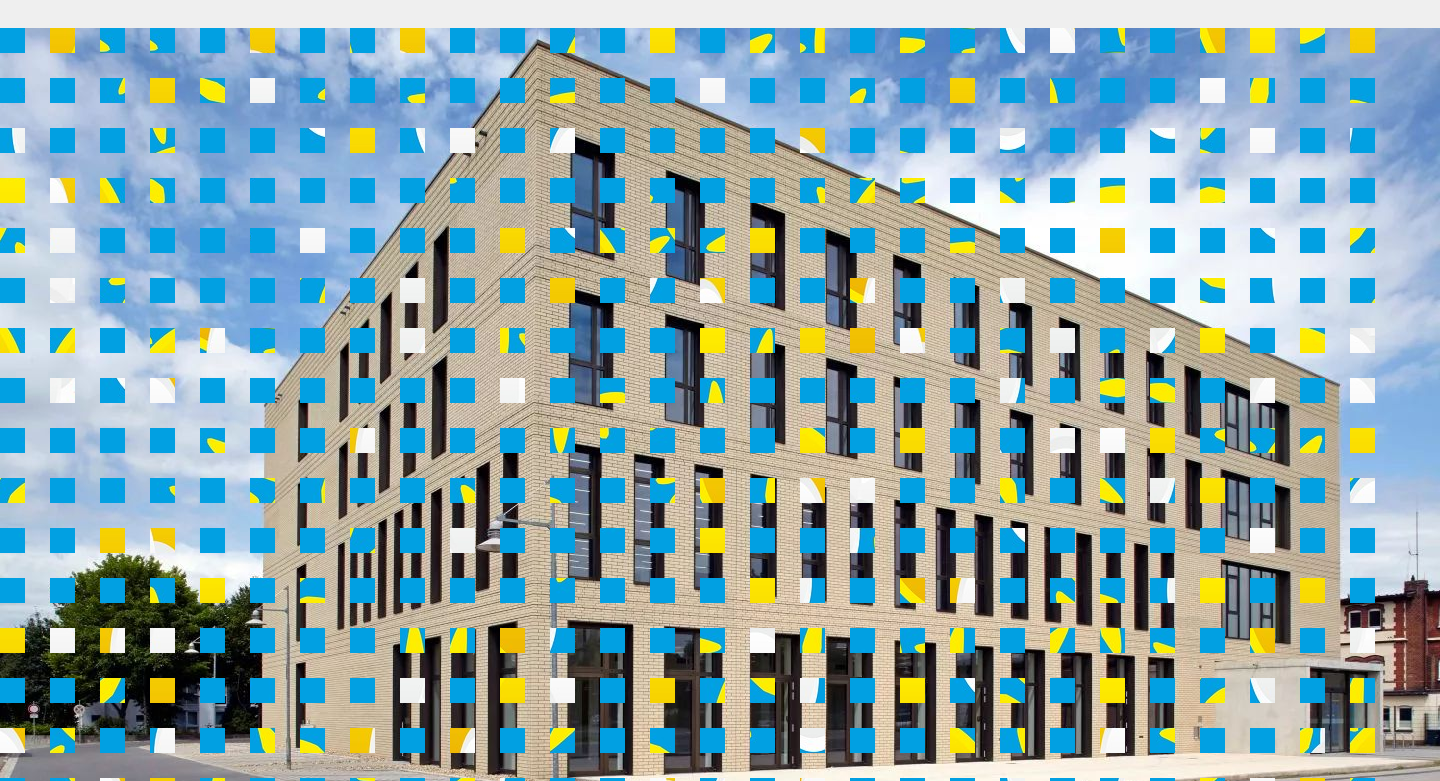
\includegraphics[width=\textwidth]{kachel_25.png}
    Ergebnisbild ($n = 25$)
  \end{minipage}
  \hfill
  \begin{minipage}{0.49\textwidth}
    \centering
    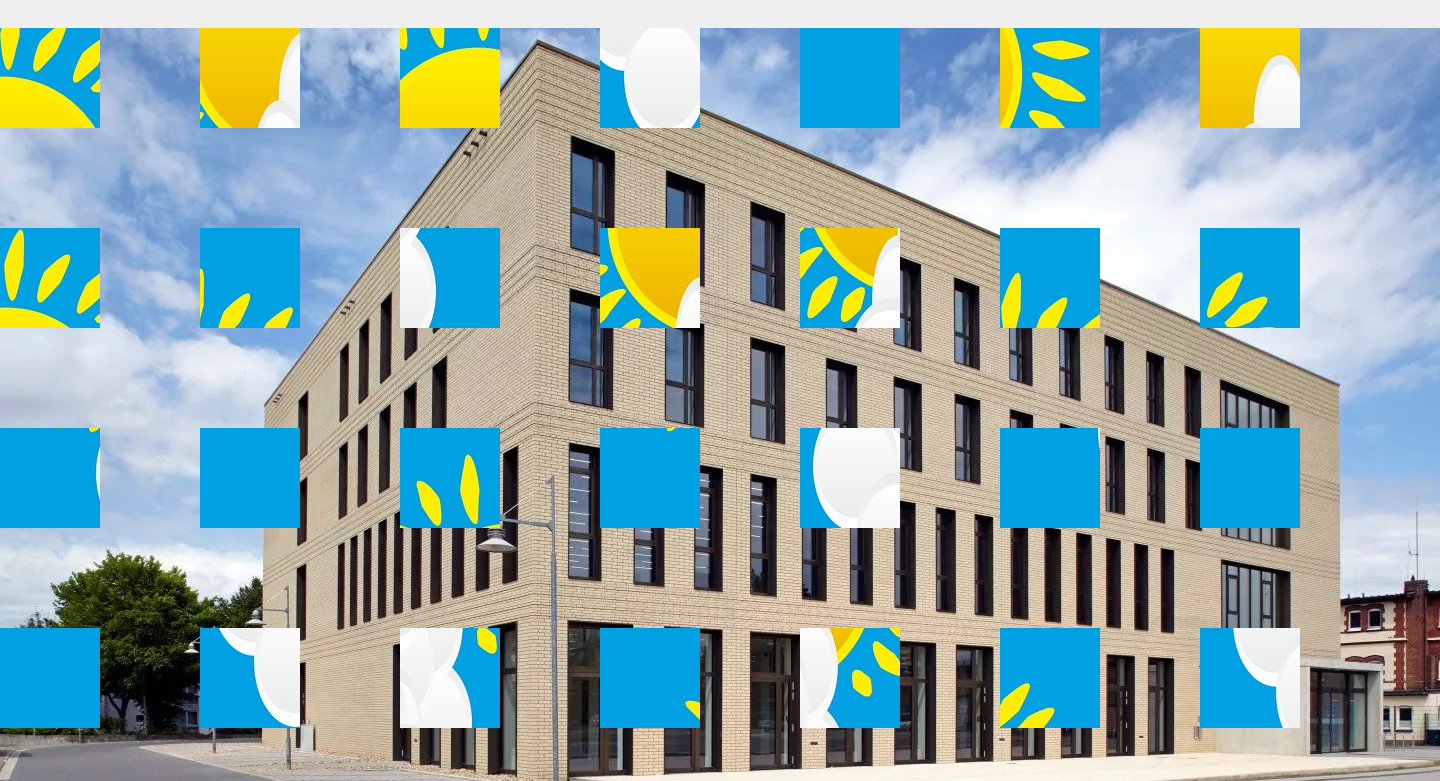
\includegraphics[width=\textwidth]{kachel_100.png}
    Ergebnisbild ($n = 100$)
  \end{minipage}
\end{figure}

\newpage

\subsection*{Teil 2: Histogrammlinearisierung}
\subsubsection*{a) Berechnung des Histogramms}
Die Berechnung des Histogramms $h_g(val)$ des Bildes $g$ wurde in der Funktion \textbf{calculate\_hist} (main.py Zeile 65) umgesetzt.

Diese Funktion erzeugt zunächst ein Array \textbf{hist} mit 256 Einträgen (da die 8-Bit-Grauwerte des Bildes zwischen 0 und 255 liegen), wobei jeder Eintrag mit 0 initialisiert wird.
Anschließend iteriert die Funktion durch jeden Punkt im Bild und inkrementiert den Wert im Array an dem Eintrag, welcher dem Werte des Punktes entspricht.
Somit ist nach der Iteration das Histogramm in dem Array \textbf{hist} gespeichert, welches zum Schluss zurückgegeben wird.

\subsubsection*{b) Berechnung des kumulativen Histogramms}
Die Berechnung des kumulativen Histogramms $H_g(val)$ aus dem Histogramm $h_g(val)$ wurde in der Funktion \textbf{cumulate\_hist} (main.py Zeile 81) implementiert.

Diese Funktion bekommt über den Parameter \textbf{hist} das Histogramm ($h_g(val)$) übergeben, und erzeugt ein neues Array \textbf{cumulative\_hist} mit der gleichen Länge wie das übergebene Histogramm und es wird eine Variable \textbf{accumulator} mit dem Wert 0 initialisiert.
Anschließend iteriert die Funktion über jeden Wert im übergebenen Histogramm und inkrementiert die Variable \textbf{accumulator} um diesen Wert, und setzt den entsprechenden Eintrag im \textbf{cumulative\_hist} Array auf den Wert der Variable \text{accumulator}.
Nach der Iteration ist das kumulative Histogramm im Array \textbf{cumulative\_hist} erstellt, welches zum Schluss zurückgegeben wird.


\subsubsection*{c) Linearisierung durch die Abbildungsfunktion $f_{eq}$ für jeden Grauwert im Bild}
Um nun mithilfe des kumulativen Histogramms die Histogrammlinearisierung durchzuführen wird eine Abbildungsfunktion $f_{eq}$ erzeugt und dieses auf jeden Punkt im Ausgangsbild angewandt.

Die Abbildungsfunktion $f_{eq}$ ergibt sich folgendermaßen:

\begin{math}
  f_{eq}(I) = \lfloor H_g(I) * \frac{K - 1}{\#Pixel} \rfloor
\end{math}

Dabei ist $H_g(I)$ das kummulierte Histogramm, $K$ die Größe des Histogramms und $\#Pixel$ die Anzahl der Pixel, welche sich aus $Länge * Breite$ des Bildes errechnen lässt.

Die Erzeugung der Abbildungsfunktion ist in der Funktion \textbf{get\_mapping} implementiert, welche über den Parameter \textbf{hist} das kumulative Histogramm übergeben bekommt. Diese Funktion gibt eine anonyme Lambda-Funktion zurück, welche die Abbildungsfunktion $f_{eq}$ implementiert.

Anschließend wird die Abbildungsfunktion auf jeden Punkt im Bild angewandt, das daraus resultierende Bild wird in der Variable \textbf{new\_img} gespeichert (main.py Zeile 141).

\newpage

\subsubsection*{Ergebnisbilder}
\begin{figure}[h]
  \centering
  \begin{minipage}{0.32\textwidth}
    \centering
    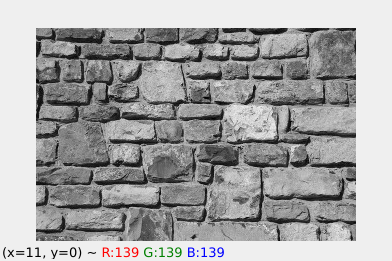
\includegraphics[width=\textwidth]{ausgangsbild.png}
    Ausgangsbild
  \end{minipage}
  \hfill
  \begin{minipage}{0.32\textwidth}
    \centering
    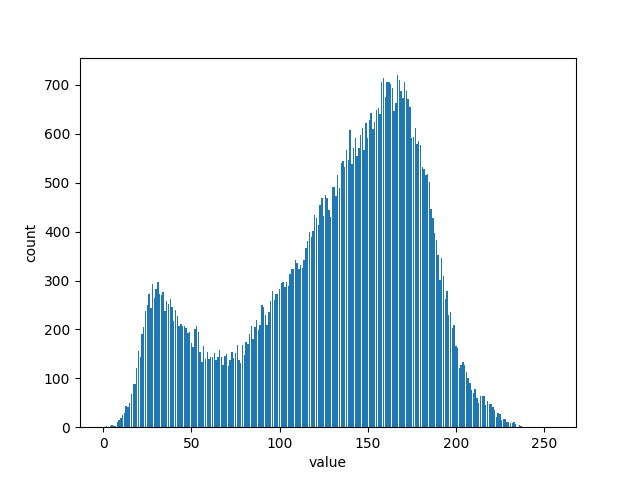
\includegraphics[width=\textwidth]{ausgangsbild_histogramm.png}
    Histogramm
  \end{minipage}
  \hfill
  \begin{minipage}{0.32\textwidth}
    \centering
    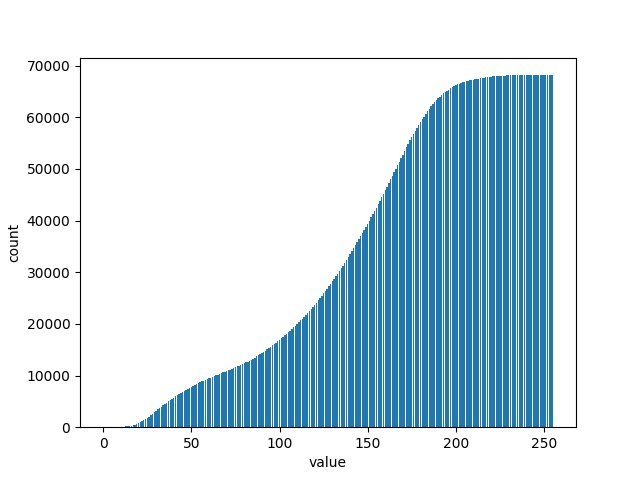
\includegraphics[width=\textwidth]{ausgangsbild_histogramm_kumulativ.png}
    kumulatives Histogramm
  \end{minipage}
\end{figure}
\begin{figure}[h]
  \centering
  \begin{minipage}{0.32\textwidth}
    \centering
    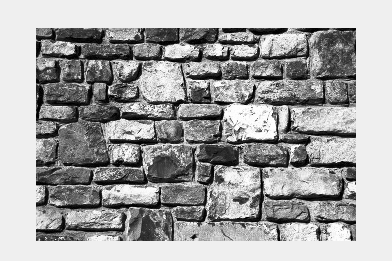
\includegraphics[width=\textwidth]{ergebnisbild.png}
    Ergebnisbild
  \end{minipage}
  \hfill
  \begin{minipage}{0.32\textwidth}
    \centering
    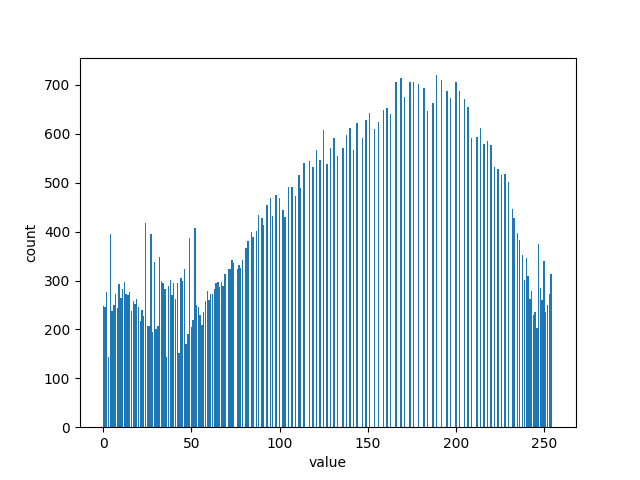
\includegraphics[width=\textwidth]{ergebnisbild_histogramm.png}
    Histogramm
  \end{minipage}
  \hfill
  \begin{minipage}{0.32\textwidth}
    \centering
    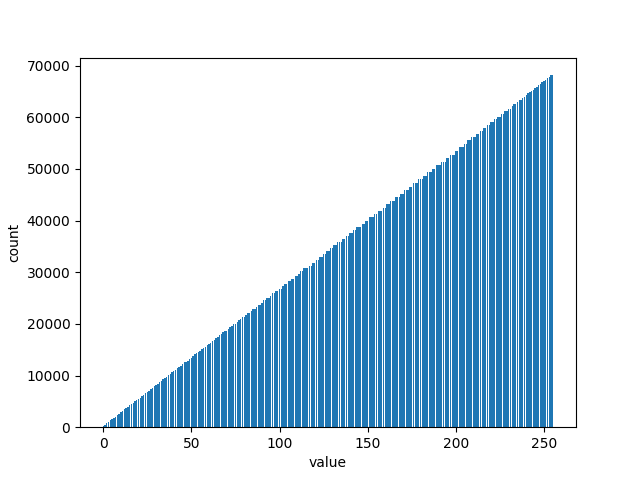
\includegraphics[width=\textwidth]{ergebnisbild_histogramm_kumulativ.png}
    kumulatives Histogramm
  \end{minipage}
\end{figure}
\begin{figure}[h]
  \centering
  \begin{minipage}{0.5\textwidth}
    \centering
    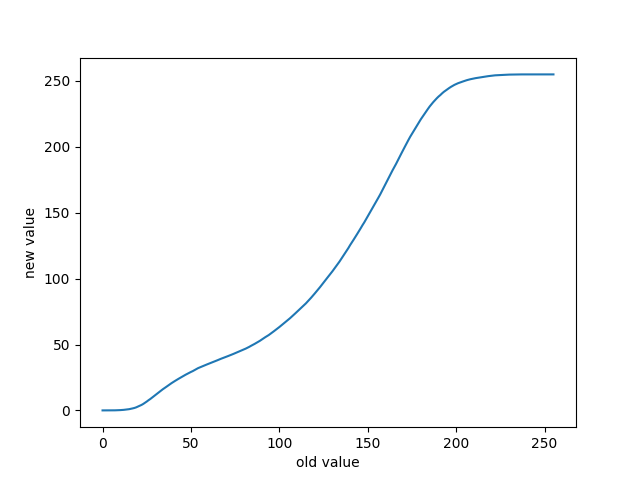
\includegraphics[width=\textwidth]{abbildungsfunktion.png}
    Abbildungsfunktion
  \end{minipage}
\end{figure}
\vfill

\end{document}
